\section{Isolating the shape assumption}\label{sec:simulation}

Proposition~\ref{prop:coupling} concerns whether the correction is
\emph{reachable}. Whether it is \emph{sound} where reachable is a separate
question, governed by~(S), and coordinate variances do not answer it. We
therefore hold the variances exactly correct and vary only the correlation
shape.

Latent curves $G\sim N(0,R_G)$ and sampling errors $S\sim N(0,\sigma^2R_S)$ are
drawn independently with $\sigma=\rho/\sqrt{1-\rho^2}$, so every coordinate
variance is correct by construction and only $R_G$ versus $R_S$ is manipulated.
The grid crosses coordinate counts $d\in\{8,24,48\}$, design shares
$\rho\in\{0.29,0.40,0.52,0.80\}$, calibration counts $K\in\{30,100,250\}$ and
five correlation pairs, at 4{,}000 replicates and nominal $90\%$: \ShapeCells{}
cells. The first and third design shares are the maxima observed at the
national and regional units in Section~\ref{sec:applications}. These are
standardised deviation vectors, not cumulative distributions and not a
finite-population design, and they supply exact scales, so the experiment
isolates~(S) from scale-estimation error and cannot bound a deployed
procedure's realised coverage.

\paragraph{The direction is predictable, and the survey-realistic direction is
the damaging one.} For a cumulative distribution function, sampling errors at
adjacent thresholds are partial sums over one sample and are strongly
positively correlated; differences between populations across thresholds carry
no such mechanism. The expected configuration is therefore noise more
correlated than latent, and this was recorded as a falsifiable prediction before
execution. It held: every structure with noise more correlated than latent
undercovers, and the reverse overcovers, reaching \ShapeReverse{} at
$\rho=0.80$, $d=48$. A matched-correlation control sits at \ShapeMatched.

\paragraph{The cost grows with coordinates, not with populations.} At
$\rho=0.80$ and $d=48$ the worst mismatch gives latent coverage
\ShapeHighDfortyeight, against \ShapeHighDeight{} at $d=8$. Raising the
calibration count does not repair it: the same cell gives \ShapeKthirty{} at
$K=30$ and \ShapeKtwofifty{} at $K=250$. The mismatch is a property of the
model, not a sampling error that more populations average away.

\begin{figure}[htbp]\centering
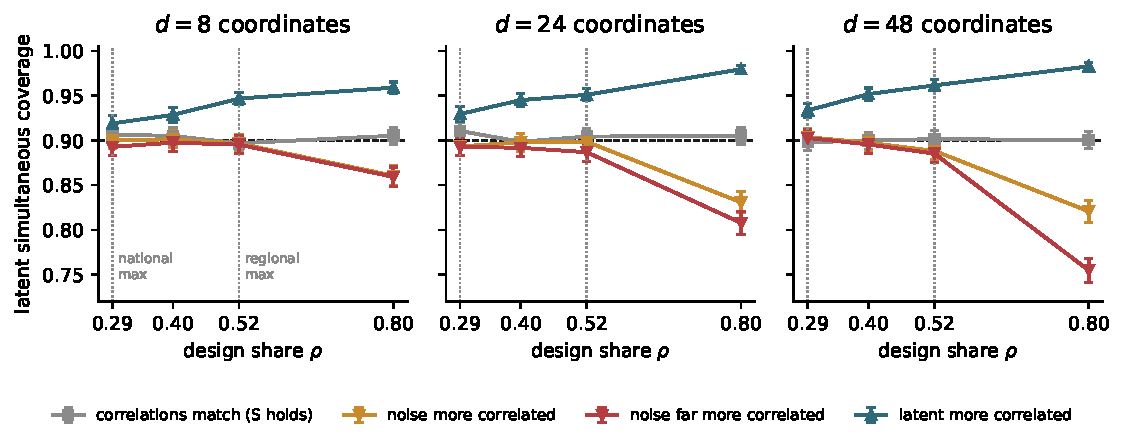
\includegraphics[width=\linewidth]{figures/shape.pdf}
\caption{Latent simultaneous coverage of the oracle scale correction with
exactly correct coordinate variances, by coordinate count, at $K=250$ and
nominal $90\%$. Bars are two Monte Carlo standard errors. Dotted verticals mark
the largest design shares observed at the national and regional
units.}\label{fig:shape}
\par\small\textbf{Alt text:} Three panels for eight, twenty-four and
forty-eight coordinates. When the two correlation structures match, coverage
stays at the nominal level throughout. When sampling error is more correlated
across coordinates than population differences, coverage falls below nominal,
mildly at the observed design shares and steeply at the highest one, and the
fall deepens as the coordinate count rises. The reverse mismatch is
conservative.
\end{figure}

\paragraph{At the observed operating points the cost is small.} At
$\rho=0.29$, the national maximum, no mismatch departs from nominal by more
than Monte Carlo error (\ShapeRealNat). At $\rho=0.52$, the regional maximum,
the cost is one to two points (\ShapeRealReg). The severe failures require
design shares above anything these surveys exhibit. The finding is therefore a
warning about direction and mechanism, not a demonstration of failure in the
applications reported here, and we state it as such.

This is a post-development sensitivity analysis, designed after inspecting the
assumption. It is exploratory, not a preregistered confirmatory test, and it
does not evaluate a deployed adaptive selector.
